\documentclass{article}

\usepackage{fancyhdr}
\usepackage[a4paper]{geometry}
\usepackage{enumerate}
\usepackage{xcolor}
\usepackage{graphicx}
\usepackage{titlesec}
\graphicspath{ {./} }
\usepackage{listings}
\usepackage{color}
\usepackage{hyperref}
\usepackage{subfigure}
\usepackage{amsmath}
\usepackage[margin=2.5cm]{caption}

\definecolor{dkgreen}{rgb}{0,0.6,0}
\definecolor{gray}{rgb}{0.5,0.5,0.5}
\definecolor{mauve}{rgb}{0.58,0,0.82}

\lstset{frame=tb,
  language=Bash,
  aboveskip=3mm,
  belowskip=3mm,
  showstringspaces=false,
  columns=flexible,
  basicstyle={\small\ttfamily},
  numbers=none,
  numberstyle=\tiny\color{gray},
  keywordstyle=\color{blue},
  commentstyle=\color{dkgreen},
  stringstyle=\color{mauve},
  breaklines=true,
  breakatwhitespace=true,
  tabsize=3
}

\setlength{\headheight}{15.2pt}
\pagestyle{fancy}
\lhead{\textbf{Structural Bioinformatics \& Python Project}}
\rhead{\textbf{Overlapy}}

\newcommand{\spaces}{\space\space\space\space\space\space}
\newcommand{\g}[1]{\textcolor[rgb]{0,0.6,0}{#1}}
\newcommand{\re}[1]{\textcolor[rgb]{0.6,0,0}{#1}}
\newcommand{\bl}[1]{\textcolor[rgb]{0,0,0}{#1}}

\begin{document}

\title{\textbf{Overlapy}\\
\begin{center}
\line(1,0){250}
\end{center}
\textit{A simple Protein Structure\\ 
Superimposer based in Python}
\begin{center}
\line(1,0){250}
\end{center}
     \author{
           \\
     \'{A}lvaro Abella Bascar\'{a}n\\
     Josep Arus Pous\\
     Samuel Miravet Verde}
     }
\maketitle

\newpage

\section*{Introduction}
The aim of this report is to explain the process and results obtained in the development of the \textit{Overlapy} program, a protein structure superimposer coded in Python 3.4, for the subjects of Structural Bioinformatics and Python of the Master in Bioinformatics (Universitat Pompeu Fabra)\\

\subsection*{\color{gray}Biological interest and Application}
The superimposition of structures (also called structural alignment) is a very useful way to establish homology between two or more polymers (e.g. proteins) based on their shape and three-dimensional conformation\cite{1}.\\

The most important features and advantages of the superimposition are:
\begin{itemize}
  \item You do not need to have prior information about the structures to align\cite{2}.
  \item It can detect evolutionary relationships even between sequences with low sequence similarity due to the fact that the biological function (and consequently the structure) is harder to alter compared to the sequence.\cite{3}.
  \item It permits to define structural motifs related with determined functions if two proteins which share function align, despite being a priori unrelated. In addition, if you have previous evolutionary information, you can detect convergent evolution to a concrete function given a structure\cite{4}.
  \item Assess the quality of a predicted structure model\cite{1}.
  \item It may help in the detection of possible biopolymers interaction (for example if a protein structurally aligns with other protein able to bind RNA) or pharmacological targets (if two proteins are very similar in structure they should share binding sites)\cite{5}. 
\end{itemize} 

\subsection*{\color{gray}Our Contribution}
Given that, having a good tool for structural alignment can be a turning point in the success of a research process. There are several programs to perform a superimposition of structures, like SuperPose\cite{6} or STAMP\cite{7}. However, we want to contribute our grain of sand with "\textit{Overlapy}", a very easy way to do superimpositions of proteins, in a user-friendly web application\cite{8} (coded in Python 3 using the Flask\cite{9}) or in an installable program\cite{10} (based on Python 3\cite{11}).

\pagebreak
\section*{Implementation}

In this section the implementation is analysed. At the end of this part, you will find a general schema of the behaviour and performance of \textit{Overlapy}.

\subsection*{\color{gray}Input Data}
The input necessary to run the program consists in two PDBs files given by the user. The program takes and processes them using the Biopython module `PDBParser' which is used to get the structure of both PDBs, later used by the principal class: Superimposer.

\subsection*{\color{gray}Selecting chains}
In order to make \textit{Overlapy} more flexible and competitive, there exists the possibility of selecting the chains to superimpose specifying them with the letter used in the PDB (for example H or L). You can set multiple selections in the same process. If the option is active, the program will only take into account those residues belonging to the chains selected.

In case of the user do not select chains, the program will take all the chains. In both situations, the implementation works in the same way, only changing the residues to superimpose.

\subsection*{\color{gray}Distances between Atoms}
Once the PDBs are loaded the first step is performed, consisting on three actions:
\begin{enumerate}
	\item The aminoacids of each protein are taken and stored (if chains are selected, it will only take those belonging to them).
	\item The list containing the residues is processed in order to extract the alpha-carbons (C$_\alpha$) and their coordinates.
	\item Finally, the function \texttt{get\_environment\_distances} computes the distances between a concrete atom and the neighbor ones determined by a radius "r", so each atom will have associated that number of distances.
\end{enumerate}

\subsection*{\color{gray}Generating a Score Matrix}
In order to get the structural alignment, the program requires a score matrix (S). It will be used to obtain the best alignment by means of a dynamic programming algorithm. That matrix, of size m x n (m=number of C$_\alpha$ considered for the first PDB; n=for the second one), will include for each pair of atoms a score value computed as:\\
$$score=\sum\limits_{i=1}^n{\mid v_i - w_i\mid}$$

Where $v$ and $w$ represent our two sets of atoms of $n$ points each one.\\

Then, if the score is small, it means that the two atoms have a similar environment, so we expect a bigger probability of match between them.


\subsection*{\color{gray}Needleman \& Wunsch algorithm}
The matrix of scores is used in this step to get the most probable alignment. To achieve this, the dynamic programming algorithm of Needleman \& Wunsch is used\cite{12}. Basically it works applying the following steps:

\begin{enumerate}
	\item A new empty matrix of \textit{Accumulated Scores} (AS) is created, adding the gap state, so the result is a matrix  (m+1 x n+1). The gap state has a penalty value `g' (1, by default).
	\item The AS matrix is filled taking the maximum value from the three results generated by the calculations (1), (2) and (3) for each position (i, j). Depending on the formula that gives the best score, a pointer for that position is stored. This step is run iteratively for i and j.
	
	\begin{center}
	\begin{tabular}{ |l|l|l| }
	\hline
	    (1)& $S_{(i,j)}+AS_{(i-1, j-1)}$ &$\nwarrow$ \\
	    (2)& $AS_{(i-1, j)}+g$ & $\leftarrow$ \\
	    (3)& $AS_{(i, j-1)}+g$ & $\uparrow$ \\   
	\hline
	\end{tabular}
	\end{center}
	
	\item Once the matrix AS is completely filled, the score of the alignment can be found in the position $AS_{nm}$. 
	\item In order to obtain the most probable alignment the program takes the path determined by the pointers starting at $AS_{nm}$ and ending at the position $AS_{1,1}$. The assignment of symbols follows:
	\begin{center}
		\begin{tabular}{ |l|l| }
		\hline
		   	$\nwarrow$ & The atoms align\\
		    $\leftarrow$ & Gap in the sequence i (vertical)\\
		    $\uparrow$ & Gap in the sequence j (horizontal)\\   
		\hline
		\end{tabular}
	\end{center}
\end{enumerate}

The alignment with gaps is part of the output generated, but in order to obtain the structural alignment we only take those pairs of atoms matching.

\subsection*{\color{gray}The Chain Order Problem}

During the development of \textit{Overlapy} we saw there were times when two very close multi-chain proteins gave wrong results, different than the expected. After several test, we found the problem was the chains order in the Needleman \& Wunsch algorithm. 

Let's suppose two related proteins with chains H and L the first and A and B the second one where we know H with A and L with B are structurally related. The structural alignment we would obtain from the scores matrices of the \textit{figure \ref{fig:nwmatrices}} could be dramatically different.

\begin{figure}[!h]
	\centering
	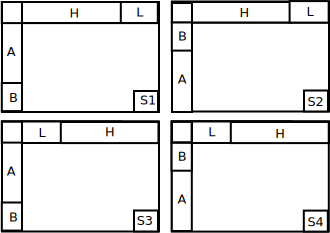
\includegraphics[scale=0.2]{images/matrices.png}
	\caption{Possible score matrices depending on the disposition of chains.}
	\label{fig:nwmatrices}
\end{figure}

If we were lucky and the residues in the PDBs were ordered by H and L, and A and B, we would obtain an alignment with score S1 and the result would be the expected and biologically significant. But what does it happen if they are not ordered?

To solve the problem, \textit{Overlapy} test all the possible combinations of chains order, performs the score matrix step for them and it takes as scores reference matrix the one that minimizes the final score (right bottom cell). That matrix will be the one that minimizes the distances between the two structures, i.e. the one that would give the best result between all the possibilities.

Finally, the Needleman \& Wunsch Associated Scores matrix is fulfilled using the best score matrix selected in the previous step.\\

That solution increase the computational cost of the algorithm only if the proteins given have more than one chain. However, even with bigger than two-chains proteins, the computational time is acceptable and it improves substantially the precision and applicability of the program. 


\subsection*{\color{gray}Obtaining the Rotation Matrix that minimizes the RMSD}
The Root-mean-square deviation (RMSD) is a measure of the average distance between the atoms of superimposed proteins. This is used as a value of the divergence from one set of atoms to another\cite{13}. Given two sets of $n$ atoms aligned $v$ and $w$, the RMSD is computed as follows:
 
$$RMSD=\sqrt{\frac{1}{n}\sum\limits_{i=1}^n{\mid\mid v_i - w_i\mid\mid^{2}}}$$

Therefore, this step takes the alignment created before by the Needleman \& Wunsch algorithm, but removing those residues pairing with a gap, in order to generate a rotation matrix $R$. This matrix, being applied to the set $w$, minimizes the RMSD (i.e. minimizes the divergence between the two sets):
$$RMSD=\sqrt{\frac{1}{n}\sum\limits_{i=1}^n{\mid\mid v_i - R w_i\mid\mid^{2}}}$$

The process followed by \textit{Overlapy} to generate the optimal rotation matrix applies the Kabsch \& Sander algorithm\cite{14}, summarized as:

\begin{enumerate}
	\item  For $v$ and $w$ the program generates two coordinate matrices (n x 3), $M_v$ and $M_w$, both including 3 columns (coordinates of the atom) and as many rows as the number of atoms in each set.
	\item \textbf{Translation:} both sets of coordinates are displaced so that the protein centroid (geometrical center) coincides with the origin of coordinates. This is done by subtracting the coordinates of the respective centroid (vector of three elements, each value computed as the mean of the elements of its column) to each atom.
	\item \textbf{Covariation Matrix:} the algorithm requires the computation of the covariation matrix $A$ as the transpose of the first by the second:
	$$A=M_{v}^{T} M_{w}$$
	\item \textbf{Generating the optimal rotation matrix:} using Singular Value Decomposition (SVD) the program returns the matrix $U$, that is, the optimal rotation matrix\cite{15}. This step is subdivided in three parts:
	\begin{enumerate}
		\item Calculate the SVD of the covariance matrix $A$ giving the matrices $V$, $S$ and $W^T$.
		$$A=VSW^T$$
		\item Decide if is needed to correct the rotation matrix to ensure a right-handed coordinate system taking the value of $d$, -1 or 1, as:
		$$ d = sign(determinant(WV^T))$$
		\item The $U$ optimal matrix comes from the calculation:
		\begin{equation*}
		    U = W\begin{pmatrix}
		        1 & 0 & 0\\
		        0 & 1 & 0\\
		        0 & 0 & d
		     \end{pmatrix} V^T
		\end{equation*}		
	\end{enumerate}
\end{enumerate}

The Kabsch \& Sander is automatically computed by \textit{Overlapy} and easily implemented thanks to the python package numpy\cite{16}, used to calculate the transposition, determinants and SVD of the intermediate matrices.

After running it, the program returns the optimal rotation matrix and the RMSD given by the one set of atoms against the second set rotated.

\subsection*{\color{gray}Rotating one of the PDBs}
The last step performed by \textit{Overlapy} takes the optimal rotation matrix and applies it to the atoms considered in one of the PDBs. With these modified coordinates along with the original coordinates from the other PDB, a new PDB is written containing the two superimposed structures, ready to be visualized in molecular visualization programs like \textit{VMD}\cite{17} or \textit{RasMol}\cite{18}.

\subsection*{\color{gray}Output generated}
In the web application as well as in the command line program, \textit{Overlapy} allows to obtain:
\begin{itemize}
	\item The best Needleman \& Wunsch alignment pairing the residues structurally more similar.
	\item The minimal RMSD for the superimposition of the two given protein.
	\item The rotation matrix that gives the minimal RMSD.
	\item A PDB containing the coordinates of the two initial structures already superimposed and ready to be visualized in molecular visualization software. 
\end{itemize}

\subsection*{\color{gray}Considerations about the Web Application}
The web application\cite{8} implements the \textit{Overlapy} program in a web interface generated and controlled by Flask\cite{9}, a framework for web development in Python.\\

\textit{Overlapy} web includes interesting features as queue control of jobs or mail advices when the job is completed, as well as all the features explained before (and in the section \textit{Improvements}). In case of having further interested on the implementation, please visit the Git repository\cite{19}.

\pagebreak
\subsection*{\color{gray}Schema of the Implementation}
The \textit{figure \ref{fig:schema}} shows in a general way, the steps implemented by \textit{Overlapy}.

\begin{figure}[h!]
	\centering
	\includegraphics[scale=0.3]{images/diagram.png}
	\caption{Workflow developed by \textit{Overlapy} in order to generate the results.}
	\label{fig:schema}
\end{figure}

\pagebreak
\section*{Tutorial on Overlapy}

\subsection*{\color{gray}Overlapy Web}
In order to use the web application of \textit{Overlapy} (\href{http://overlapy.undeadpixels.net/}{http://overlapy.undeadpixels.net/}), you just need to load the two PDBs you want to compare, set the chains to select (by default it takes all the chains present, please, be careful with chains that do not belong to the protein (e.g. I)), give your email and run it.

You will be redirected to a `job' page that will show the form input and a message telling your task is not completed. In any case you will promptly receive an email telling you can go to the `job' page and access your results. In general the program works fast so you could wait in the web too.

In case the process goes wrong, the page will show an error message. If this occurs, please contact the developers will receive and they will try their best in order to solve your problem.

\subsection*{\color{gray}Installation}
If you want to use \textit{Overlapy} locally, first of all, you have to install the program. To do this, go to the \texttt{setup.py} directory and type:

\lstset{language=bash}
\begin{lstlisting}
sudo python3 setup.py install
\end{lstlisting}

Once you have done this, you will have \textit{Overlapy} installed in your computer and executable with the name \texttt{overlapy}.

\subsection*{\color{gray}Basic Usage}
This section shows a generic usage example. If you want to see \textit{Overlapy} in action, see the next section: `Examples of usage'
The basic help can be displayed in the terminal by typing
\lstset{language=bash}
\begin{lstlisting}
overlapy -h
\end{lstlisting}
or
\lstset{language=bash}
\begin{lstlisting}
overlapy --help
\end{lstlisting}

If you type this, you will be able to see there exists several arguments you can use; between all of them, only three are necessary by default:
\begin{center}
	\begin{tabular}{ |l|l| }
		\hline
		   	-i1 & first input filename, in PDB format\\
		    -i2 & second input filename, in PDB format\\
		    -o & output filename, in PDB format\\   
		\hline
	\end{tabular}
\end{center}

So we could run a basic \textit{Overlapy} just typing:
\lstset{language=bash}
\begin{lstlisting}
overlapy -i1 protein1.pdb -i2 protein2.pdb -o protein1protein2.pdb
\end{lstlisting}

This will generate a PDB file containing the two initial structures superimposed (stored the input 1 as chain A and chain B for the second) and will show in your terminal:
\begin{itemize}
	\item The best Needleman \& Wunsch alignment pairing the residues structurally more similar.
	\item The minimal RMSD for the superimposition of the two given protein.
	\item The rotation matrix that gives the minimal RMSD.
\end{itemize}

If you want to store all this information in files, you can use three additional arguments:
\begin{center}
	\begin{tabular}{ |l|l| }
		\hline
		   	-m & store the rotation matrix, in \texttt{tsv} format\\
		    -r & generate a text file containing the minimized RMSD\\
		    -a & save the alignment in clustal format\\   
		\hline
	\end{tabular}
\end{center}

\subsection*{\color{gray}Selecting Chains}
\textit{Overlapy} also allows you to perform the superimposition only over selected chains of your proteins. To do this, it provides to additional arguments:
\begin{center}
	\begin{tabular}{ |l|l| }
		\hline
		   	-c1 & Chains selected from the first PDB\\
		    -c2 & Chains selected from the second PDB\\
		\hline
	\end{tabular}
\end{center}

For this function take into account two considerations:
\begin{itemize}
\item Provide the chains to use with one letter code (H, L, A, B...).
\item If you want to take more than one chain in a PDB, write the letters without spaces (e.g. HL).
\item In case you only select chains in one PDB, the other will be taken completely. 
\item In general, be careful with proteins containing non-proteic elements like inhibitors. They are considered `chains' in the PDB so if you use them the alignment will be wrong. 
\end{itemize}

Then, we could run \textit{Overlapy} selecting chains using:
\lstset{language=bash}
\begin{lstlisting}
overlapy -i1 protein1.pdb -c1 HL -i2 protein2.pdb -c2 A -o protein1protein2.pdb -a -m
\end{lstlisting}

With that command we will find the best superimposition of the chains H and L of the first PDB and the chain A of the second one. The PDB output will be stored in the \texttt{protein1protein2.pdb} file. Two extra files, containing the matrix and the alignment, will be generated as we have activate the `-a' and `-m' options; the RMSD will be displayed in the terminal.

\section*{Specific Examples}

\subsection*{\color{gray}An easy one: Thioredoxins}

To see \textit{Overlapy} in action, we are going to start superimposing the thioredoxin of human and the one of \textit{Drosophila melanogaster}. That protein contains only a chain and participates in essential antioxidant and redox-regulatory processes via a pair of conserved cysteine residues\cite{20}.

We download the two proteins from \texttt{www.rcsb.org/pdb/home/} using their protein codes: 3TRX for the human thioredoxin and 1XWC for the fly one (the files are also available in the `pdbs' folder of the repository). In order to obtain the superimposition, we run:
\begin{lstlisting}
overlapy -i1 1XWC.pdb -i2 3TRX.pdb -o thioredoxins.pdb -a -m -r
\end{lstlisting}

This generates a pdb called \texttt{thioredoxins.pdb} containing the superimposition. The result can be visualized in the \textit{figure \ref{fig:super}} using \textit{RasMol}\cite{18}, displaying by ribbons and coloring by chain: chain A (first file, fly thioredoxin) in purple and chain B (human one) in green.

\pagebreak

\begin{figure}[h]
	\centering
	\subfigure[view 1]{
	\includegraphics[width=.4\textwidth]{images/superposition1.png}}
	\subfigure[view 2]{
	\includegraphics[width=.4\textwidth]{images/superposition2.png}}
	\caption{Two views in RasMol for the superimposition of fly and human thioredoxins using \textit{Overlapy}.}
	\label{fig:super}
\end{figure}
In addition three extra files are generated: 1) structural alignment in clustal format, 2) rotation matrix in tsv format and 3) a plain text file containing the RMSD (\textit{figure \ref{fig:alignmatrix}}).
\begin{figure}[h!]
	\centering
	\subfigure[Structural Alignment]{
	\includegraphics[width=.8\textwidth]{images/alignment.png}}
	\subfigure[Rotation Matrix]{
	\includegraphics[width=.8\textwidth]{images/matrix.png}}
	\subfigure[RMSD]{
		\includegraphics[width=.2\textwidth]{images/rmsd.png}}
	\caption{Structural alignment, rotation matrix and RMSD for fly and human thioredoxins superimposition using \textit{Overlapy}.}
	\label{fig:alignmatrix}
\end{figure}

As we can see, thanks to the superimposition we are able to assert that the 3TRX and 1WXC are really structurally similar, thing that makes sense with the fact they have the same function. 

\pagebreak

\subsection*{\color{gray}One step further: Subtilisins}
Subtilisins belong to subtilases, a group of serine proteases, initially described in \textit{Bacillus subtilis}. In addition to be a key element in several bacterial pathogenic processes, they are a common tool in molecular biology\cite{21}.

Let's consider we are interested in study the structural homology of several known-structure subtilisines. For example, 1SBH and 1SCJ, both from \textit{Bacillus subtilis}. We obtain a very bad result (RMSD=6.23) if we run a basic \textit{Overlapy} (Note as we do not activate -r, -m and -a options the alignment, rotation matrix and RMSD will be displayed by the terminal):

\begin{lstlisting}
overlapy -i1 1SBH.pdb -i2 1SCJ.pdb -o subtilisins.pdb
\end{lstlisting}

And the superimposed PDB obtained shows how it seems the 1SCJ have two chains and only one could be superimposed to 1SBH (\textit{figure \ref{fig:subti}}) and the second chain of 1SCJ is generating some noise displacing the whole protein to an incorrect result.

\begin{figure}[!h]
	\centering
	\includegraphics[scale=0.6]{images/subti1.png}
	\caption{1SBH(blue) superimposed with the 1SCJ(orange)}
	\label{fig:subti}
\end{figure}

We can use the chain selection option of \textit{Overlapy} to see if our assumptions are correct. As 1SBH only have one chain, we only have to select the chain A for the 1SCJ.

\begin{lstlisting}
overlapy -i1 1SBH.pdb -i2 1SCJ.pdb -c2 A -o subtilisins.pdb
\end{lstlisting}

And this time we obtain a very good structural alignment with a RMSD of 0.44 (\textit{figure \ref{fig:subtis}}).

In reality, 1SBH and 1SCJ are the same protein, but 1SBH is the processed subtilisin, we use this structures as an example of the correct performance of the option `chains' as we have obtained the expected result.

\begin{figure}[h]
	\centering
	\subfigure[view 1]{
	\includegraphics[width=.4\textwidth]{images/subti2.png}}
	\subfigure[view 2]{
	\includegraphics[width=.4\textwidth]{images/subti3.png}}
	\caption{Two views in RasMol for the superimposition of two different subtilisins using \textit{Overlapy}.}
	\label{fig:subtis}
\end{figure}

\subsection*{\color{gray}Reliability of the results}
In order to see if our results are reliable, we compare them with the ones obtained replicating the superimposition of thioredoxins (1WXWC and 3TRX) by SuperPose web version\cite{22}.

For this concrete case, we obtain a RMSD of 1.51, very similar to our 1.16 given by \textit{Overlapy} for the same case. In addition, the superimposed PDB result (\textit{figure \ref{fig:superpose}}) is almost exactly the same compared with the \textit{Overlapy} result.

\begin{figure}[!h]
	\centering
	\includegraphics[scale=0.4]{images/superpose.png}
	\caption{3TRX(red) superimposed with the 1XWC(blue) using SuperPose.}
	\label{fig:superpose}
\end{figure}

Regrettably, \textit{SuperPose} web do not give the structural alignment and the rotation matrix so we cannot compare them. However, it seems that at least \textit{Overlapy} works returning similar results to those obtained by \textit{SuperPose}. 

\pagebreak
\section*{Future improvements}
Some interesting complementary options we are interested in trying to implement are:
\begin{itemize}
	\item Include the option to select the $C_{\beta}$ instead of the $C_{\alpha}$. That approach presents a special advantage: it takes into account the rotameric state of each residue as well as its location along the backbone. In order to solve the problem the glycine does not have $C_{\beta}$ we could use the $C_{\alpha}$ or virtualize  the $C_{\beta}$ for it. 
	\item Include the possibility of adding from which amino acid to which other the superimposition is going to be restrained.
	\item The implementation based on Needleman \& Wunsch will always return an alignment, even if the structures are absolutely distant. It would be interesting to add a kind of "check" in order to give a confidence or reliability value to the user, for instance, set a minimum sequence similarity.
	\item Try to adapt the implementation in order to be able to perform superimposition of RNA structures, as made by some projects\cite{23}. This could give us information about the importance of the three-dimensional structure of RNA in some fields like expression, cell response or mutation, as well as finding possible homology relations between structure and function of RNAs.

\end{itemize}
  
\section*{Conclusion}
We have developed from scratch a fully usable program: \textit{Overlapy}, capable of superimposing protein structures. It is able to generate coherent and reliable results from two PDBs, giving an unique PDB with the two structures superimposed in addition to files containing the structural alignment, the rotation matrix and the RMSD in case you need it.

Despite having used Biopython and Numpy to deal with PDB parsing and linear algebra operations, we have fully implemented the algorithm needed to do the superimposition (Needleman \& Wunsch and Kabsch \& Sander).

Finally, \textit{Overlapy} is presented in three different flavours:
\begin{enumerate}
\item Web application: user-friendly web \cite{8} that wants to simplify the life of those researchers that only want a direct and easy to use structural aligner application.
\item Command line tool: an installable program you can download and use locally in your terminal. Simple and useful to integrate in bigger pipelines and scripts.
\item Python library: ready to be included as part of bigger programs.
\end{enumerate}

\pagebreak


\begin{thebibliography}{8}
\bibitem{1}
Zhang, Y.; Skolnick, J. (2005). "The protein structure prediction problem could be solved using the current PDB library". Proc Natl Acad Sci USA 102 (4): 1029–34.

\bibitem{2}
Sippl, M.; Wiederstein, M. (2012). "Detection of spatial correlations in protein structures and molecular complexes". Structure 20 (4): 718–728.

\bibitem{3}
Godzik, A. (1996). "The structural alignment between two proteins: Is there a unique answer?". Protein science : a publication of the Protein Society 5 (7): 1325–38.

\bibitem{4}
Jana, B.; Morcos, F.; Onuchic, JN.(2014). "From structure to function: the convergence of structure based models and co-evolutionary information". Phys Chem. 16 14):6496-507.

\bibitem{5}
Petras, J.; Ilya, A. (2013). "Global and local structural similarity in protein–protein complexes: Implications for template-based docking". Proteins: Structure, Function, and Bioinformatics. 81 12):2137–2142.

\bibitem{6}
\href{http://wishart.biology.ualberta.ca/SuperPose/}{http://wishart.biology.ualberta.ca/SuperPose/}

\bibitem{7}
\href{http://www.compbio.dundee.ac.uk/manuals/stamp.4.2/}{http://www.compbio.dundee.ac.uk/manuals/stamp.4.2/}

\bibitem{8}
\href{http://overlapy.undeadpixels.net/}{http://overlapy.undeadpixels.net/}

\bibitem{9}
\href{http://flask.pocoo.org/}{http://flask.pocoo.org/}

\bibitem{10}
\href{https://github.com/SMV818VMS/overlapy}{https://github.com/SMV818VMS/overlapy}

\bibitem{11}
\href{https://www.python.org/download/releases/3.0/}{https://www.python.org/download/releases/3.0/}

\bibitem{12}
Needleman, S.B.; Wunsch, C.D. (1970). «A general method applicable to the search for similarities in the amino acid sequence of two proteins». Journal of molecular biology (Elsevier) 48 (3): 443–453.

\bibitem{13}
Maiorov VN, Crippen GM (1994). "Significance of root-mean-square deviation in comparing three-dimensional structures of globular proteins". J Mol Biol 235 (2): 625–634.

\bibitem{14}
Kabsch, W. (1976) "A solution for the best rotation to relate two sets of vectors", Acta Crystallographica 32:922.

\bibitem{15}
Golub, G. H.; Kahan, W. (1965). "Calculating the singular values and pseudo-inverse of a matrix". Journal of the Society for Industrial and Applied Mathematics: Series B, Numerical Analysis 2 (2): 205–224. 

\bibitem{16}
\href{http://www.numpy.org/}{http://www.numpy.org/}

\bibitem{17}
\href{http://www.ks.uiuc.edu/Research/vmd/}{http://www.ks.uiuc.edu/Research/vmd/}

\bibitem{18}
\href{http://rasmol.org/}{http://rasmol.org/}

\bibitem{19}
\href{https://github.com/undeadpixel/overlapy_web}{https://github.com/undeadpixel/overlapy\_web}

\bibitem{20}
Wollman E, d'Auriol L, Rimsky L, Shaw A, Jacquot J, Wingfield P et al. (October 1988). "Cloning and expression of a cDNA for human thioredoxin". J. Biol. Chem. 263 (30): 15506–12.

\bibitem{21}
Ottesen Mm, Svendsen I (1970). "The subtilisins". Methods Enzymol. 19: 199–215.

\bibitem{22}
http://wishart.biology.ualberta.ca/SuperPose/

\bibitem{23}
Hoksza, D.; Svozil, D. (2012). "Efficient RNA pairwise structure comparison by SETTER method". Bioinformatics 28 (14): 1858–1864.

\end{thebibliography}


\end{document}
